%!TEX root = ../tex/TheShorthPlot.tex
%$Id: TheShorthPlot.Rnw.tex 44 2007-10-07 20:01:08Z gsawitzki $
% -*- mode: noweb; noweb-default-code-mode: R-mode; -*-
%
%         TheShorthPlot
%  
%  Adjust the path names below and run the R command to process this file
%
% enc<-options(encoding="MacRoman")
% #enc<-options(encoding="")
% oldoptions<-options(width=72,prompt=">", continue="+")
% oldoptions<-options(width=72,prompt="  ", continue="  "); setwd("/Users/gs/projects/rforge/lshorth/tex/"); Sweave(file= "../Rnw/TheShorthPlot.Rnw.tex", output="TheShorthPlot.tex", debug=TRUE, eps=FALSE);options(oldoptions)
%

%global flags for conditional builds
%:flags
\def\private{true}% comment out for public version
\def\solutions{true}% comment out to hide solutions
\def\usehyperref{true}% comment out to skip hyperref

\ifx\pdfoutput\undefined % We're not running pdftex
\documentclass[dvips,12pt,a4paper,twoside]{amsart}
\else
%\documentclass[pdftex,12pt,a4paper,twoside]{amsbook}
\documentclass[pdftex,12pt,a4paper,twoside]{amsart}
\usepackage{thumbpdf}
\pdfcompresslevel=9
\fi

%\usepackage{harvard}
\usepackage{graphicx}
%\DeclareGraphicsRule{.tif}{png}{.png}{`convert #1 `dirname #1`/`basename #1 .tif`.png}
\graphicspath{{./}{./graphics/}{./media/}{./Rnw_out}}%Graetzer, p. 420
\usepackage[english]{babel}%hyphenation must be after babel
\usepackage[applemac]{inputenc}

%\RequirePackage{makeidx}
\usepackage{gssdaart}

\newcommand{\idef}[1]{%index definition entry, not shown in text
\label{#1}\index{#1|textbf}}
\newcommand{\iref}[1]{%index reference entry, reference shown in text
\ref{#1}\index{#1}}

\ifx\private\undefined%
\typeout{******** gssda: ommitting private info ********}
\newcommand{\gsnote}[1]{}
\else
\newcommand{\gsnotestyle}{\textcolor{green}}
\newcommand{\gsnote}[1]{\marginpar{\textcolor{green}{#1}}}%abstract base method
\fi


\title[The Shorth Plot]{The Shorth Plot\\\tiny{Technical Report}}
\author{G\"unther Sawitzki}
\address{G\"unther Sawitzki\newline
StatLab Heidelberg\newline
Im Neuenheimer Feld 294\newline
D 69120 Heidelberg}%\\\bigskip\bigskip\bigskip\bigskip\bigskip \\ %
\thanks{\ifx\private\undefined%
\typeout{ommitting private stuff ********}
\else
\emph{Private Version}\\
\fi
}
\email{gs@statlab.uni-heidelberg.de}
\urladdr{http://lshorth.r-forge.r-project.org/}
\keywords{shorth, distribution diagnostics, data analysis, probability mass concentration}

\date{June 1992, published as technical report \cite{gs92shrth}.\\
For quotation, please use the general reference \cite{gs94oned}.\\
Revised: August 2007\\
Typeset, with minor revisions: \today}                                           % Activate to display a given date or no date

%:layout parameters
\setlength{\parskip}{12pt}
\setlength{\parindent}{0pt}
\setkeys{Gin}{width=0.9\textwidth}

\makeindex

\usepackage{/Library/Frameworks/R.framework/Versions/2.6/Resources/share/texmf/Sweave}
\begin{document}
\begin{abstract}
We introduce the shorth plot for exploratory diagnostics of distributions. The shorth plot is a graphical representation of the length of the shorth, the shortest interval covering a certain fraction of the distribution. Localising the shorth, i.e. requiring it to contain specific data points, makes it usable for diagnostics.

The shorth can be defined as a functional which has an immediate empirical version. The empirical length of the shorth converges to the theoretical value with rate $n^{-\frac{1}{2}}$.
\end{abstract}

\maketitle
%\frontmatter
%\shorttableofcontens{}{1}
\begingroup
\setlength{\parskip}{0pt}
\tableofcontents
\endgroup
%\mainmatter
\section{Distribution Diagnostics}
Exploratory diagnostics is one of the basic tasks in data analysis. Graphical displays are essential tools. If the task can be narrowed down, specialised displays may be available. For example, if there is a model distribution $F$ to be compared with, from a mathematical point of view the empirical distribution $F_n$ is a key instrument, and its graphical representations such as 
$PP$-plots $$x \mapsto \left(F \left(x\right),F_n \left(x \right) \right)$$ 
or $QQ$-plots $$\alpha \mapsto \left(F^{-1} \left(\alpha\right),F_n^{-1} \left(\alpha \right) \right)$$ are tools of first choice. If we consider  the overall scale and location, box \& whisker plot is a valuable tool. This tool loses its sharpness for large data sets, as the rules for identifying ``out'' and ``far out'' points seem to reflect data sizes which were typical at the time box \& whisker plots were introduced, but this is a detail which might be fixed. The main limitation is that  box \& whisker plots give a global view and ignore any local structure. In particular, they are not an appropriate tool if it comes to analyse the modality of a distribution. More specialised tools are needed in this case, such as the silhouette and the excess density plot, both tools introduced in \cite{dwmgs91jasa}.

Here we look for general purpose tools for the analysis of a distribution.
While we have some instruments for specific tasks, the situation is not satisfactory if it comes to general purpose tools. $PP$-plots and $QQ$-plots need considerable training to be used as diagnostic tools, as they do not highlight qualitative features. 

Focussing on the density, in contrast to the distribution function, leads to density estimators and their visual representations, such as histograms and kernel density plots. These however introduce another complexity, such as the choice of cut points or bandwidth choice. The qualitative features revealed or suggested by density estimation based methods may critically depend on bandwidth choice. Moreover, estimating density is a more specific task than understanding the shape of a density. Density estimation based methods are prone to pay for the initial smoothing steps in terms of slow convergence or large fluctuation, or disputable choices of smoothing.

We will use the length of the shorth to analyse the qualitative shape of a distribution. The shorth is the shortest interval containing half of a distribution. The length of the shorth is a functional which is easy to estimate, with convergence of rate $n^{-\frac{1}{2}}$, and gives a graphical representation which is easy to interpret. 

We will start with the classical definition of a shorth. To overcome the handicaps of other methods, we have to extend the classical definition to supply localisation, and to allow for multi scale analysis.

%
\section{The Length of the Shorth}
The shorth is the shortest interval containing half of a distribution. More general, the $\alpha$-shorth is the the shortest interval containing an $\alpha$ fraction of the distribution. The shorth was originally introduced in the Princeton robustness study as a candidate for a robust location estimator, using the mean of a shorth as an estimator for a mode \cite{ANDREWSD1972Robust-Estimati}. 

As a a location estimator, it performed poorly. The mean of a shorth as an estimator of
location has an asymptotic rate of only $n ^{-1/ 3}$,
with non-trivial limiting
distribution. 
\cite[p. 50]{ANDREWSD1972Robust-Estimati}  \cite[p. 767]{Shorack1986Empirical-proce}. Moreover, the shorth interval is not well defined, since there may be several competing intervals. 


However, as Gr�bel \cite{grbl88lshrt} has pointed out, the length of the shorth has a convergence rate of $n^{-\frac{1}{2}}$ with a Gaussian limit. The critical conditions are that the shorth interval is sufficiently pronounced (see \cite[section 3.3]{grbl88lshrt}).  Essentially this means that the shorth interval must not be in a flat part of the distribution. While the shorth position is not a good candidate as a location estimator, the length of the shorth qualifies as a reasonable candidate for scale estimation.

%:def: shorth
The length of the shorth is a functional which can be localised, thus providing a tool for local diagnostics.
We define:
\begin{dfn} The shorth length  at point $x$ for coverage level $\alpha$ is
$$
S_\alpha(x)=  \min \{|I|: I=[a,b],\  x \in I,\  P(I) \geq \alpha\}.
$$ 
\label{dfn:shrth}
\end{dfn}

We get the length of the shorth as originally defined by taking $\inf_{x}S_{0.5}(x)$.

The definition has a functional form which can be applied to theoretical as well as empirical distributions. The definition in terms of a theoretical probability $\prob{\noop}$ has an immediate empirical counterpart, the empirical length of the shorth
$$
S_{n, \alpha}(x)=  \min \{|I|: I=[a,b],\   x  \in I,\  P_n(I) \geq \alpha\}
$$ 
where  $\prob[n]{\noop}$ is the empirical distribution.

The get a picture of the optimisation problem behind the shorth length, we consider the bivariate function
$$
a,b \longmapsto I = [a,b] \longmapsto \big( \left| I \right|, P\left(I\right) \big)\qquad \text{where } a \leq b.
$$
This is defined in the half space $a \leq b$ above the diagonal. The level curves of $ \left| I \right|$ are deterministic parallels to the diagonal. The level curves of $P(I)$ depend on the distribution. The shorth at level $\alpha$ minimises $\left| I \right|$ in the area above the level curve at level 
$\alpha$, i.e. $\prob{I} \geq \alpha$. Going to the empirical version replaces the level curves of of $P(I)$ by those of  $P_n(I)$. 
The theoretical curves for the Gaussian distribution and for a  Gaussian sample are shown in figure \ref{fig:level}.
 Localising the shorth at a point $x$ restricts optimisation to the top left quadrant anchored at $a=b=x$.
 
\gsnote{paragraph added}The increasingly flat level curves for $P([a,b]) = const$  in figure \ref{fig:level} illustrate why the location of the shorth does not have satisfactory stattistical properties while the length of the shorth has good asymptotic behaviour.

\todo{align scales for plots where reasonable}
\begin{figure}[htb]
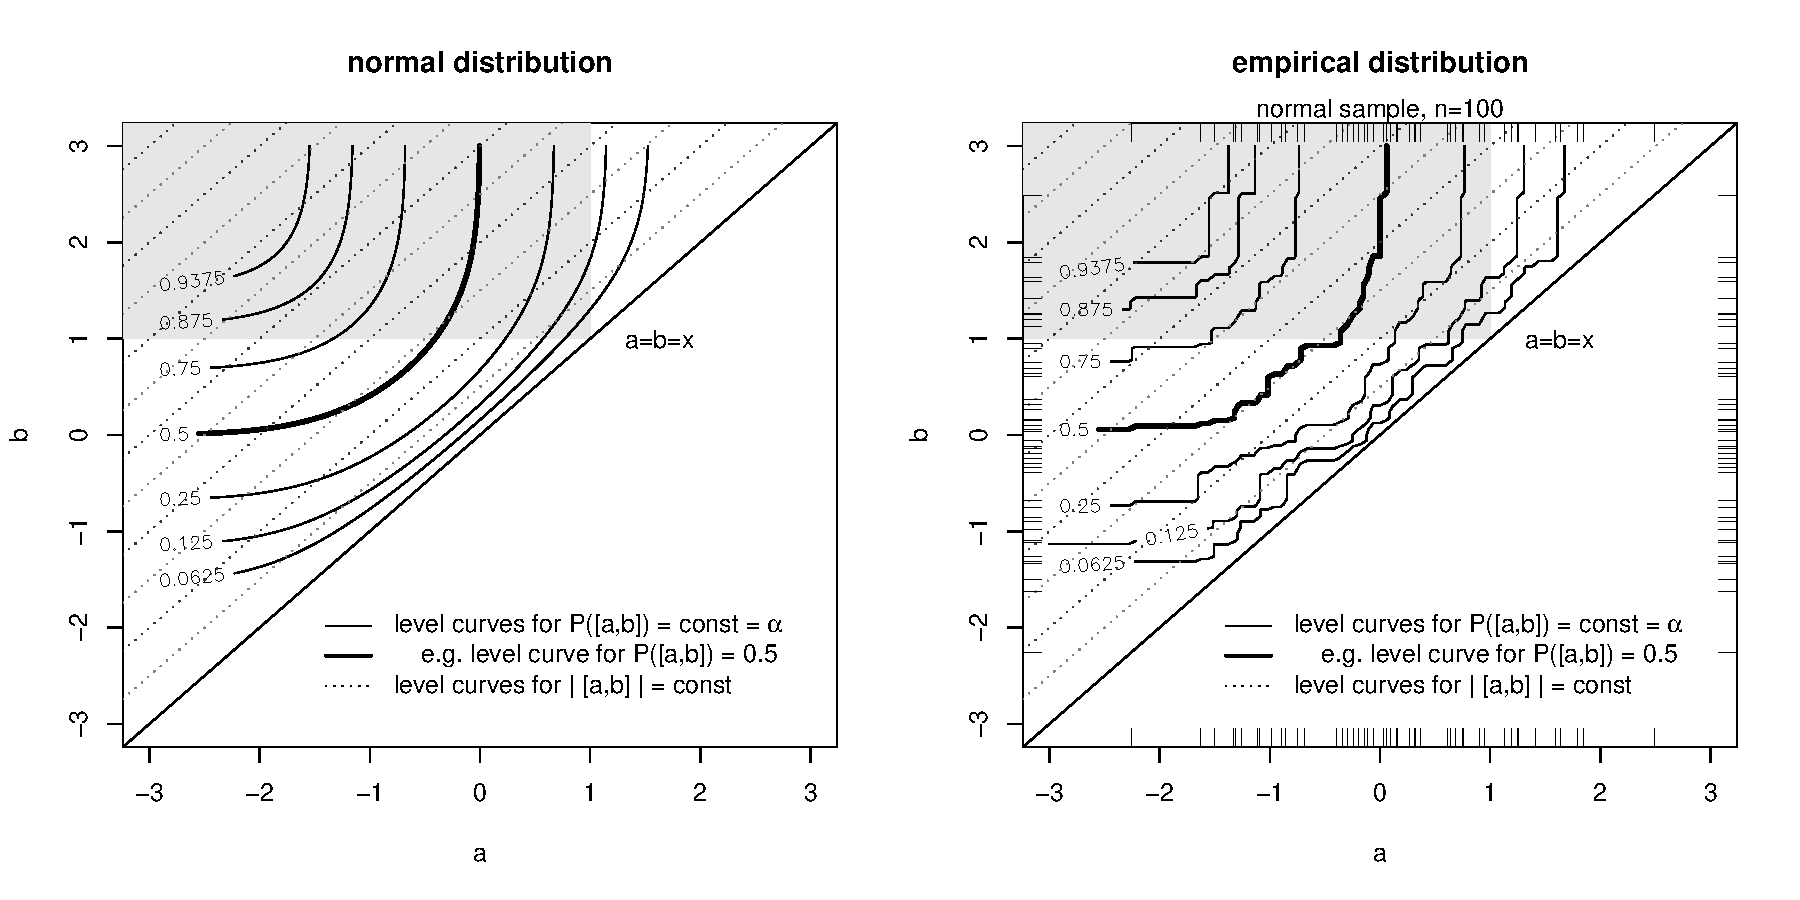
\includegraphics[width=1.0\linewidth]{TheShorthPlot-level}
\caption{The shorth length as an optimisation problem: minimize $| [a,b] |,$ 
under the restriction $P([a,b] ) \geq \alpha$. Localising at $x$ restricts the optimisation  to the quadrant top left of $x$ (shaded grey).}
\label{fig:level}
\end{figure}

\todo{inverse or dual?}
The inverse optimisation problem is to find the maximal coverage which can be achieved by a given length:
$$
\delta \longmapsto \sup  \{P(I): | I | \geq \delta \}
$$
%\delta \longmapsto \sup_{y}  \{P(I): | I | \geq \delta \}
together with its localised and/or empirical version.
%
The relation between the shorth length and its inverse is extensively used in Gr\"ubel's analysis of the asymptotics  of the (unlocalised) shorth. A modified version of Gr\"ubel's proof carries over to the localised shorth, provided there are no flat parts in the distribution, giving a  $n^{-\frac{1}{2}}$ asymptotics of the empirical shorth length to the theoretical shorth length.
\todo{extend discussion of concentration function}

\subsection{Elementary Properties}
Here and in the following, we assume a sample $X_1, \ldots, X_n$ from some distribution $P$ with 
distribution function $F$. Let $P_n$ be the empirical distribution and $F_n$ the empirical distribution 
function. The $k$-th order statistics is denoted by $X_{(k)}$.

\chck{ok?}\begin{rem}\emph{(invariance)}
For all $\alpha$
$$
x \mapsto S_\alpha(x)
$$
is invariant under shift transformations and equivariant under scale transformations, that is for $x^\prime 
= a  x+b$, for the transformed shorth length $S^\prime$ we have
$$
{S^\prime}_{\alpha}(x^\prime) = a  S_\alpha(x).
$$
\end{rem}
%
\begin{rem}\emph{(monotonicity)}\label{rem:monot}
For all $x$, 
$$
\alpha \mapsto S_\alpha(x)
$$
is monotonously non decreasing in $\alpha$.
\end{rem}
%
%: continuous F
%

If $F$ is continuous with  density $f$, additional properties are guaranteed:

\begin{rem}\emph{(minimising intervals)}
If $F$ is continuous, then for any $\alpha \in [0, 1]$ and any $x \in \real{}$, there is a (possibly infinite) 
interval $I$ such that $x \in I$, $\prob{I} = \alpha$ with $|I| = S_{\alpha}(x)$. \newline
If $\alpha < 1$, the interval is
finite and contained in $[x-S_{\alpha}(x), x+ S_{\alpha}(x)]$.
\end{rem}
\todo{add proof concl. 5}

\begin{rem}\emph{(continuity)}
For a continuous distribution function $F$,
$$
(x,\alpha) \mapsto S_\alpha(x)
$$
is continuous.
\end{rem}
%
\begin{rem}\emph{(strict monotonicity)}\label{rem:monotone}
For a continuous distribution function $F$, for each $x \in \real{}$,
$$
(x,\alpha) \mapsto S_\alpha(x)
$$
is strictly increasing in $\alpha$ on $(0, 1)$.
\end{rem}


In the limit,  $\lim_{\alpha \rightarrow 0} S_\alpha(x) =0$. 

In particular, for the empirical version, $S_{n, 
\alpha}(x) =0$ for $\alpha \leq \frac{1}{n}$.

%
%
\subsection{Computing the Empirical Shorth Length}
To use empirical distribution functions, the discontinuous case is of interest.

\begin{rem}\emph{(interpolation)}\label{rem:interpolation}
If $x_0 < x < x_1$ and $\prob{\ \left( x_0, x_1 \right)\  }=0$, then 
$$S_{\alpha}(x) = \big(S_{\alpha}\left(x_0\right) + \Delta_0\big) \wedge 
\big(S_{\alpha}\left(x_1\right) + \Delta_1\big),$$
where $x= x_0 + \Delta_0 = x_1 - \Delta_1$.
\end{rem}
%
\begin{rem}\emph{(algorithm)}\label{rem:algo}
For $\alpha, 0 \leq \alpha \leq 1,$ let 
$$\Delta_{\alpha} = \min\left\{k: \frac{k+1}{n} \geq \alpha\right\}.$$
Then
$$
S_{n,\alpha}(X_{i})= \min \{X_{(j+\Delta_{\alpha}} - X_{(j)} : \ 1 \leq j \leq i \leq j+\Delta_{\alpha} \leq n\}.
$$
Using a stepwise algorithm, a further reduction of complexity is possible: 
let 
$$\msc{C}_i \deq \{ I : X_{(i)} \in I, \prob{I} \geq	 \alpha\}$$
be the set of candidate intervals at $X_{(i)}$ for level $\alpha$. 
Then
$$S_{n,\alpha}(X_{i}) = \min\{|I|: I \in \msc{C}_i \}.$$
Unless boundary corrections apply, we have
$$\msc{C}_i = \msc{C}_{i-1} \setminus \{ [X_{(i-1-\Delta_{\alpha})}, X_{(i-1)}] \} 
\cup \{ [X_{(i)}, X_{(i+\Delta_{\alpha}})] \}.$$ 
This gives an algorithm with linear complexity in $n$.

\end{rem}

An additional reduction is possible using the monotonicity in $\alpha$ (remark \ref{rem:monotone}), but this may not be worth the effort.
%
%
%
\section{The Shorth Plot}
\begin{dfn}
The shorth plot is the graph of 
$$x \mapsto S_\alpha(x)$$
 for a selection of coverages $\alpha$.
\end{dfn}

The empirical shorth plot is $$x \mapsto S_{n,\alpha(x)}.$$ See figure \ref{fig:shorthdef}.
\begin{figure}[htb]
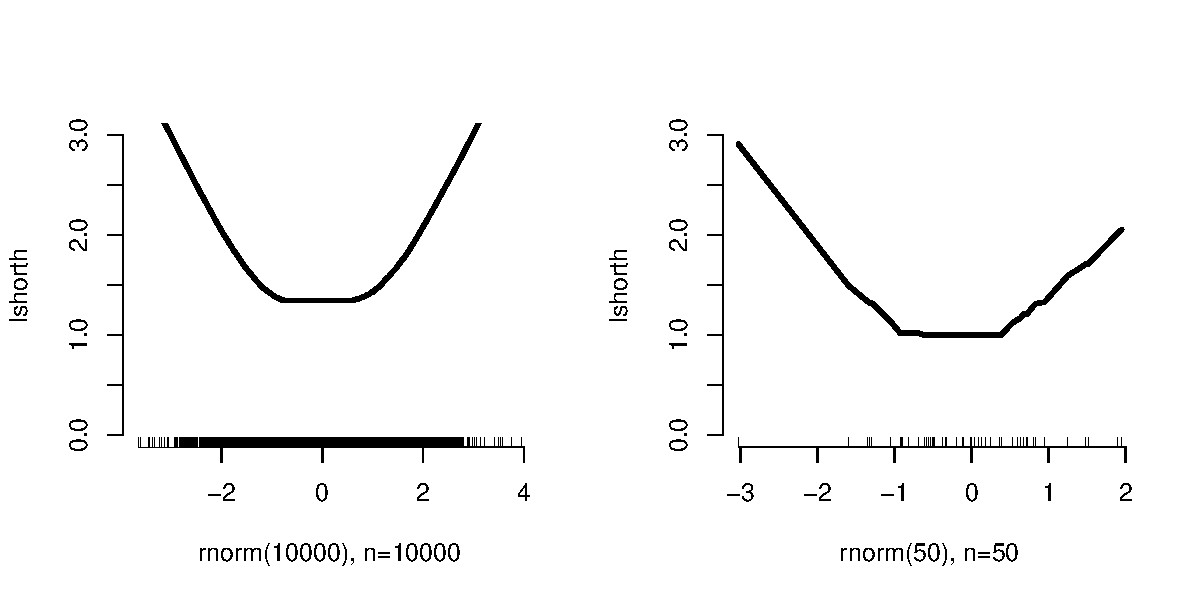
\includegraphics[width=1.0\linewidth]{TheShorthPlot-shorthdef}
\caption{Theoretical shorth length and shorth length for a sample of 50 normal variates for $\alpha=0.5$. Note: different scales are used.}
\label{fig:shorthdef}
\end{figure}


Mass concentration now can be represented by the graph of $x \mapsto S_\alpha(x)$. A
small length of the shorth signals a large mass concentration. To make the interpretation easier, we 
prefer to invert the orientation of the axis so that it is aligned with density axis. This will be used in the subsequent figures.


\subsection{Display Details}
%
Several choices can to be made for the visual representation. 
The common conception seems to view a distribution represented by its density. From a mathematical 
point of view, plotting $x \mapsto 1/S_{\alpha}(x)$ would be first choice, since this is approximately 
proportional to the local average density.  This however is an infinitesimal approximation. It tends to overemphasise peaks (see figure \ref{fig:sinv}), and becomes useless for point masses. Using just a downward orientation for the y-axis 
avoids the need to special case point masses while keeping the qualitative impression.
\begin{figure}[htb]
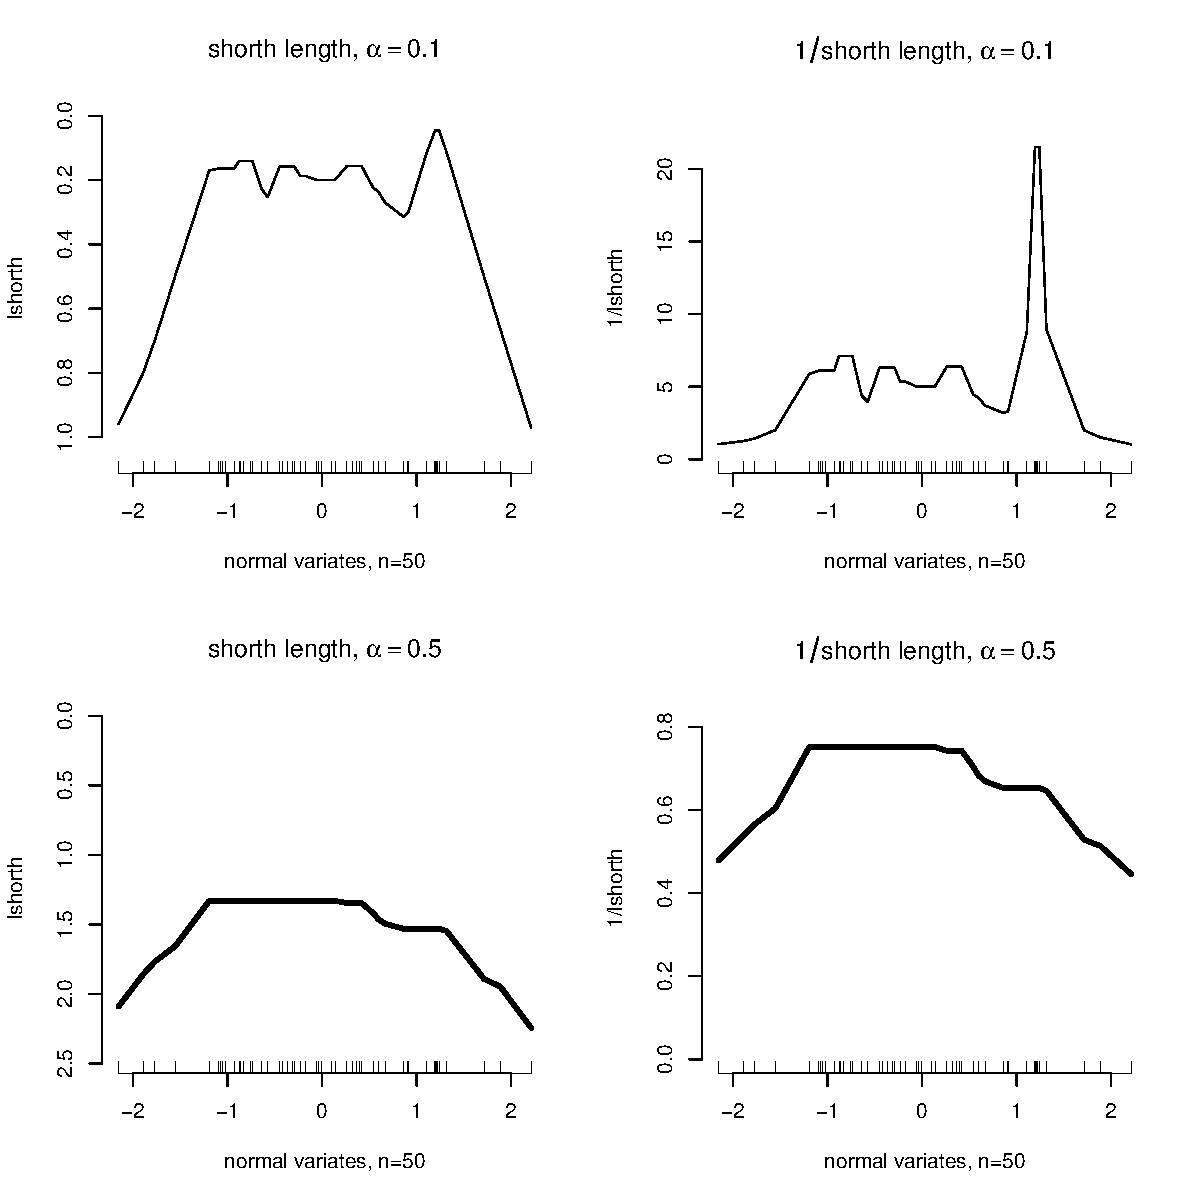
\includegraphics[width=1.0\linewidth]{TheShorthPlot-sinv}
\caption{Shorth length (left) and 1/Shorth length (right) for a sample of 50 normal variates. The axis for the shorth is pointing downward. Note: different scales are used.}
\label{fig:sinv}
\end{figure}
%

To make comparison between different data sets easier, we can use the classical shorth length $\min_x S_{0.5}(x)$ as a scale estimator and remove the scale dependency by taking the quotient. This quotient
$$x \mapsto\  \ \frac{S_{\alpha}(x)}{\min_{x^\prime} S_{0.5}(x^\prime)}$$
is called the  standardised short length .
%for the (standardised) shorth plot. 
The only difference is the scale labeling.
%\begin{figure}[htb]
%<<fig=TRUE, echo=FALSE,label=sstd, height=4, width=8, include=FALSE>>=
%oldpar<-par(mfrow=c(1,2))
%lshorth(rnorm50, rescale="none", probs=0.5, frame.plot=FALSE,  legend=NULL, main=NULL)
%lshorth(rnorm50, rescale="std", probs=0.5, frame.plot=FALSE,  legend=NULL, main=NULL)
%par(oldpar)
%@
%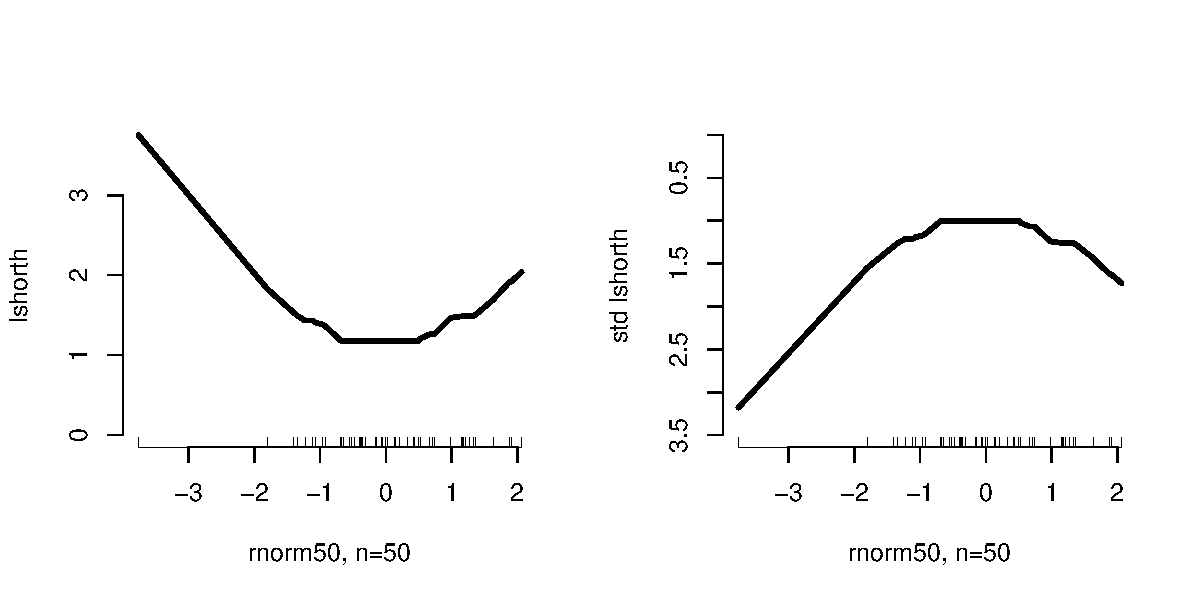
\includegraphics[width=1.0\linewidth]{TheShorthPlot-sstd}
%\caption{Shorth length and standardised shorth length for the same sample of 50 normal variates as above ($\alpha=0.5$).}
%\label{fig:sstd}
%\end{figure}
In these notes, we do not use standardized shorth length, but use the original scales.


Instead of the exact interpolation
as in remark \ref{rem:interpolation}, we use a linear interpolation. The loss of information is negligible. 

%Figure \ref{fig:s05theor} gives examples of the shorth plot for the theoretical uniform, normal and log-normal distribution.\todo{mc so far}
Figure \ref{fig:s05unln} gives examples of the shorth plot for the uniform, normal and log-normal distribution with varying sample sizes.
%
%\begin{figure}[htb]
%<<fig=TRUE, echo=FALSE,label=s05theor, height=3, width=6, include=FALSE>>=
%oldpar <-par(mfrow=c(1,3))
%lshorth(runif(1000), probs=0.5,  rescale="neg", frame.plot=FALSE, legend="topright", ylim=c(-1,0), xlab="uniform", main=NULL)
%lshorth(rnorm(1000), probs=0.5,  rescale="neg", frame.plot=FALSE,  legend = NULL, xlab="normal", main=NULL)
%lshorth(exp(rnorm(1000)), probs=0.5,  rescale="neg", frame.plot=FALSE,  legend = NULL, xlab="log normal", main=NULL);
%par(oldpar)
%@
%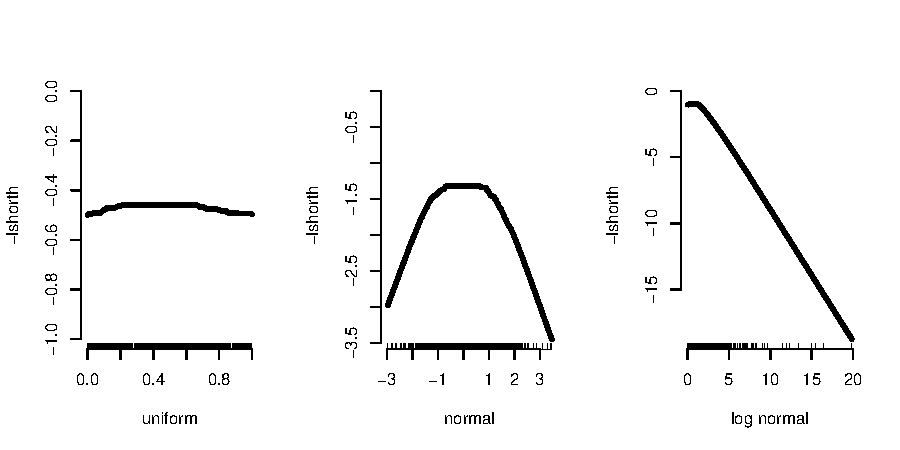
\includegraphics[width=1.0\linewidth]{TheShorthPlot-s05theor}
%\caption{ $x \mapsto - \ S_{n, {0.5}}(x)$
%%\caption{ $x \mapsto - \ \frac{S_{0.5}(x)}{\min_{x\prime} S_{0.5}(x\prime)}$ 
%for a uniform, a normal, and a log-normal distribution
%Note: Different scales are used for the shorth length.}
%\label{fig:s05theor}
%\end{figure}
%
%
\todo{legend to bottomleft?}
\begin{figure}[htb]
% for Tilburg paper
%lognormal<- exp(rnorm(n)); lshorth(lognormal, probs=ps,  rescale="neg", frame.plot=FALSE,   legend ="topright", main=NULL);
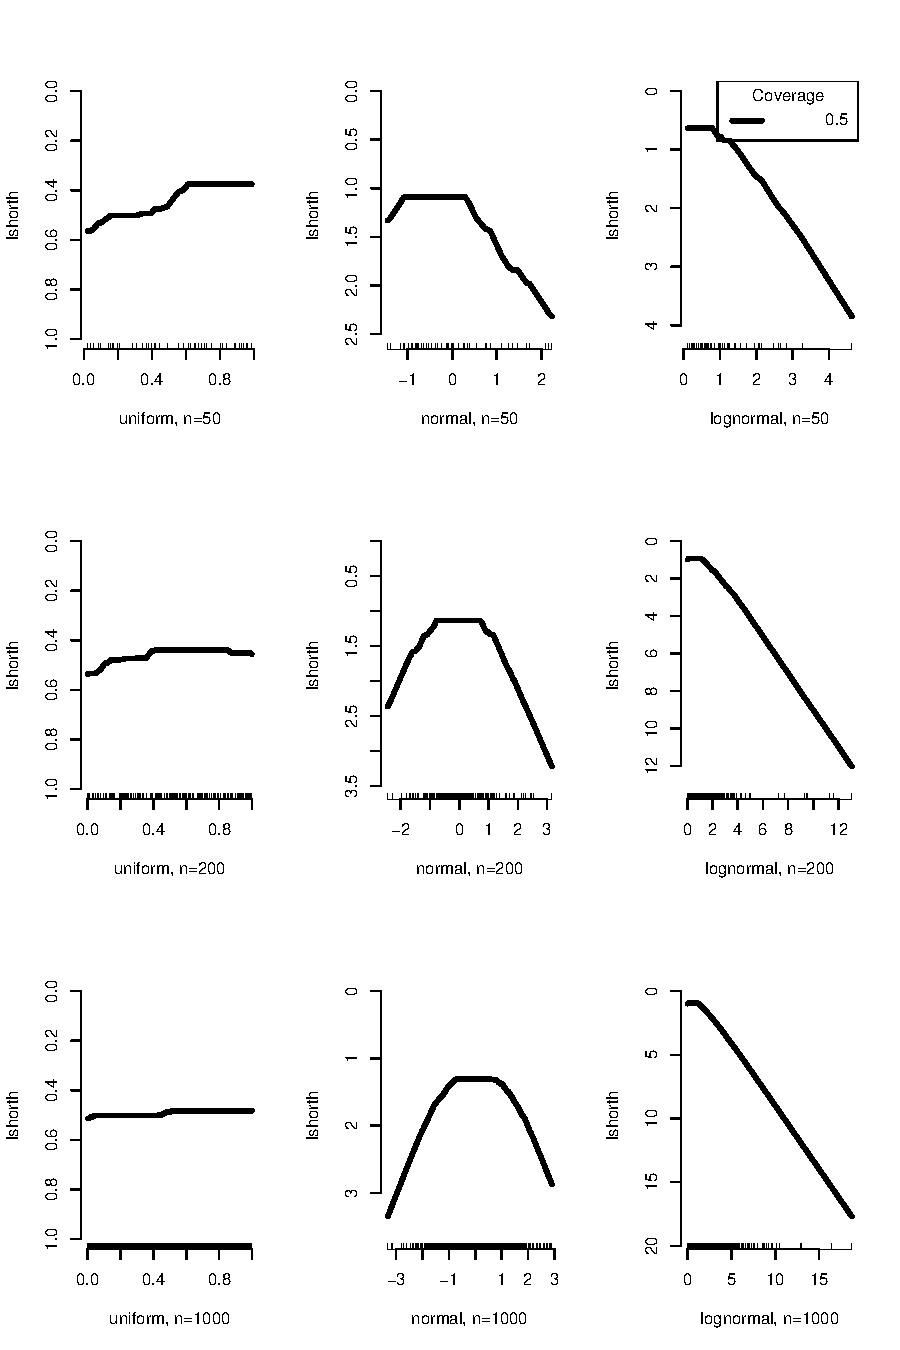
\includegraphics[width=1.0\linewidth]{TheShorthPlot-s05unln}
\caption{ $x \mapsto  \ S_{n,{0.5}}(x)$
%\caption{ $x \mapsto - \ \frac{S_{0.5}(x)}{\min_{x\prime} S_{0.5}(x\prime)}$ 
for a uniform, a normal, and a log-normal distribution with varying sample sizes.
Note: Different scales are used for the shorth length.}
\label{fig:s05unln}
\end{figure}
\todo{replace last line by theoretical plots}

Varying the coverage level $\alpha$ as in figure \ref{fig:s05unlnalpha} gives an impression of the mass concentration. Small coverage levels (the top curves in figure  \ref{fig:s05unlnalpha}) give information about the local behaviour, in particular near modes. High coverage levels give information about skewness the overall distribution shape. A dyadic scale with steps chosen based on the sample size, e.g., $0.125, 0.25, 0.5, 0.75, 0.875$,  is a recommended choice. The monotonicity (remark \ref {rem:monot}) allows the multiple  scales to be displayed simultaneously without overlaps, thus giving a multi resolution image of the distribution.

%
%\begin{figure}[htb]
%<<fig=TRUE, echo=FALSE,label=s05theoralpha, height=3, width=6, include=FALSE>>=
%oldpar <-par(mfrow=c(1,3))
%ps <- c(0.125,0.25,0.5,0.75,0.875)
%lshorth(runif(1000), probs=ps,  rescale="neg", frame.plot=FALSE, legend="topright",  ylim=c(-1,0), xlab="uniform", main=NULL)
%lshorth(rnorm(1000), probs=ps,  rescale="neg", frame.plot=FALSE,  legend = NULL, xlab="normal", main=NULL)
%lshorth(exp(rnorm(1000)), probs=ps,  rescale="neg", frame.plot=FALSE,  legend = NULL, xlab="log normal", main=NULL);
%par(oldpar)
%@
%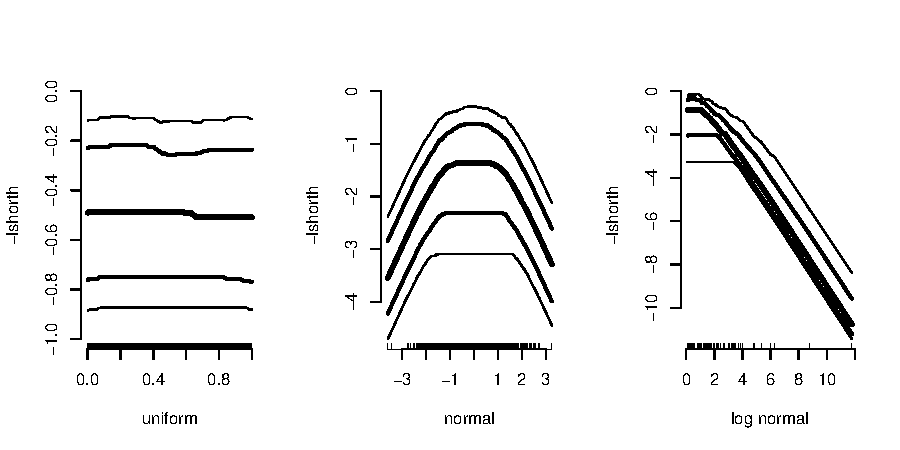
\includegraphics[width=1.0\linewidth]{TheShorthPlot-s05theoralpha}
%\caption{ $x \mapsto - \ S_{n, {0.5}}(x)$
%%\caption{ $x \mapsto - \ \frac{S_{0.5}(x)}{\min_{x\prime} S_{0.5}(x\prime)}$ 
%for a uniform, a normal, and a log-normal distribution
%Note: Different scales are used for the shorth length.}
%\label{fig:s05theoralpha}
%\end{figure}
%\todo{mc so far}
%
\begin{figure}[htb]
% for tilburg paper
%\caption{ $x \mapsto 1/S_{\alpha}(x)$ for a uniform, a normal and a log-normal distribution with sample sizes
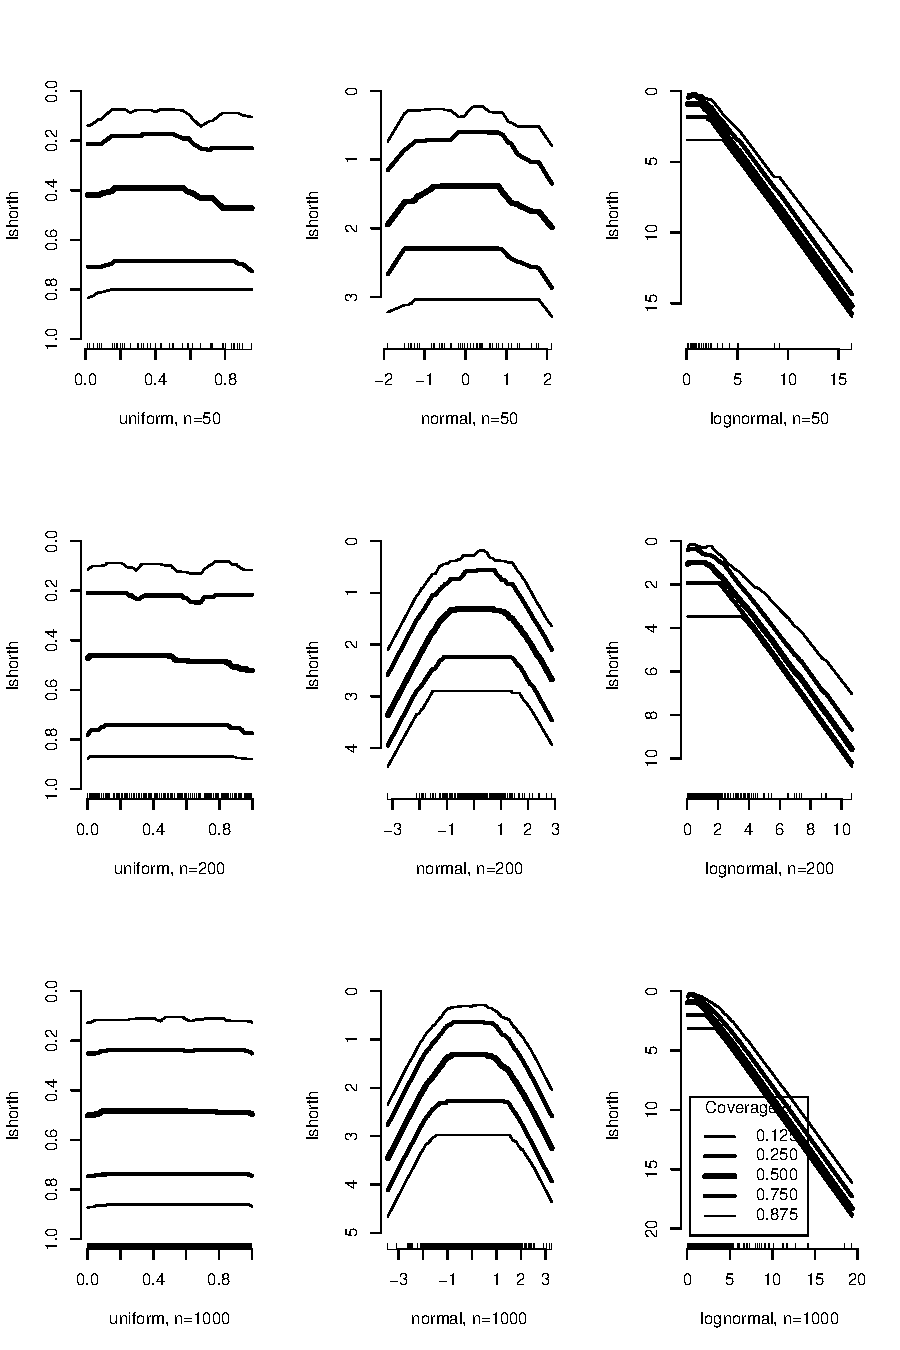
\includegraphics[width=1.0\linewidth]{TheShorthPlot-s05unlnalpha}
%\caption{ $x \mapsto - \ \frac{S_{\alpha}(x)}{\min_{x\prime} S_{0.5}(x\prime)}$
\caption{ $x \mapsto  \ S_{n, \alpha}(x)$
 for a uniform, a normal and a log-normal distribution with varying sample sizes.}
%$50, 100, 200$.}
\label{fig:s05unlnalpha}
\end{figure}
\todo{replace 10000 by theor}
%
%
\clearpage
%
%
\section{Examples}
%
\subsection{Old Faithful Geyser}
%
As a first example, we use the eruption durations of the Old Faithful geyser. The data is just one component of a bivariate time series data set. 
Looking at a one dimensional marginal distribution ignores the process structure. However these data have been used repeatedly to illustrate smoothing algorithms (figure \ref{fig:faithfuldens}), and we reuse it to illustrate our approach (see figure \ref{fig:faithful}). This is a good-natured data set showing two distinct nodes  with sizeable observation counts, and some overall skewness.


%\begin{figure}[htb]
%\begin{minipage}0.4\linewidth
%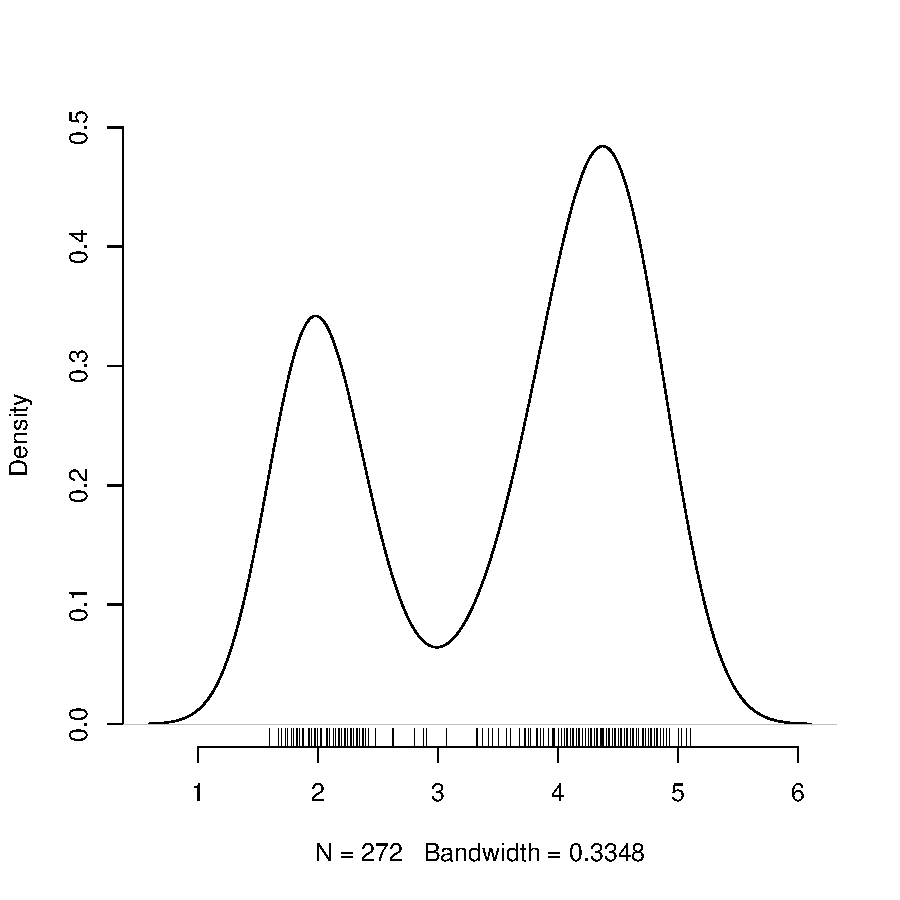
\includegraphics[width=0.5\linewidth]{TheShorthPlot-Faithfuldens}
%\caption{Eruption durations of the Old Faithful geyser: density estimation (R defaults)}\label{fig:faithfuldens}
%\end{figure}
%\end{minipage}
%%
%\begin{minipage}0.4\linewidth
%\begin{figure}[htb]
%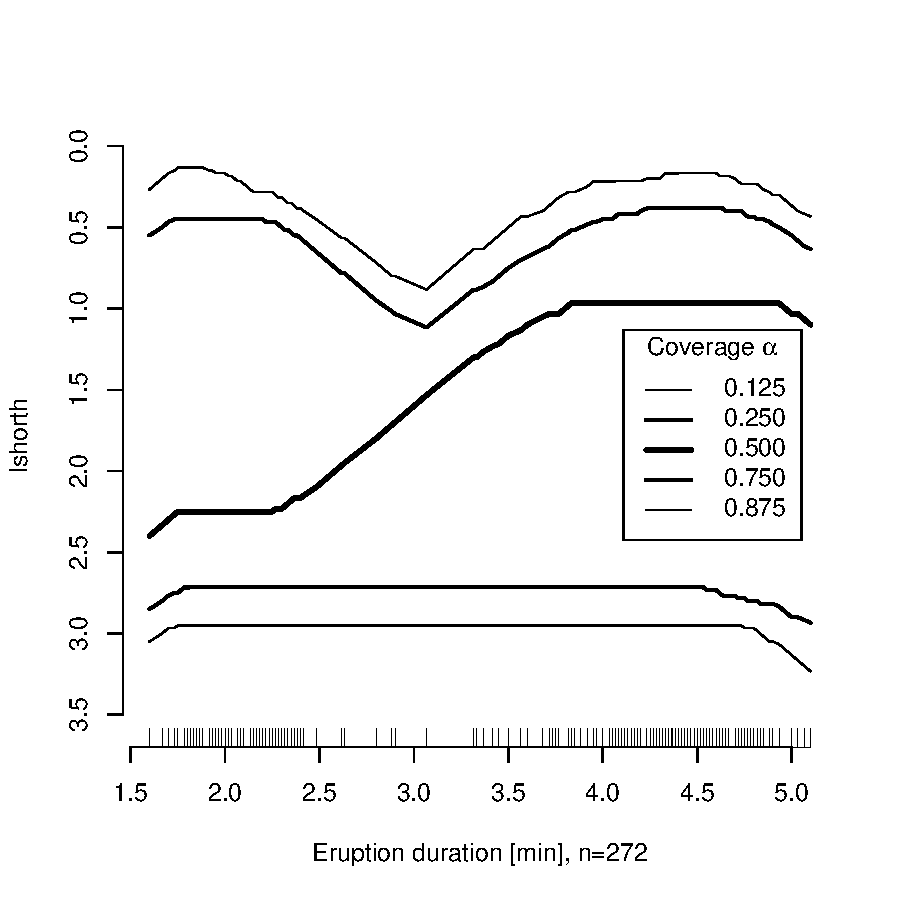
\includegraphics[width=0.5\linewidth]{TheShorthPlot-Faithful}
%\caption{Eruption durations of the Old Faithful geyser: shorth plot}\label{fig:faithful}
%\end{figure}
%\end{minipage}
\begin{figure}[htb]
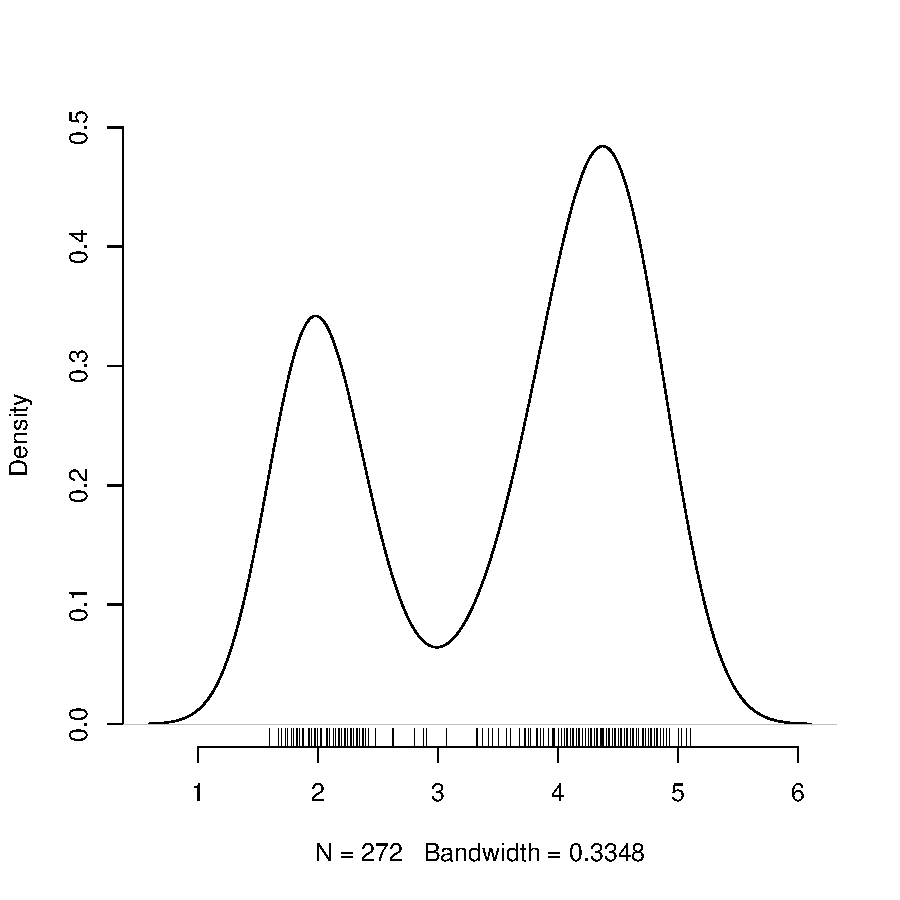
\includegraphics[width=0.45\linewidth]{TheShorthPlot-Faithfuldens}
%\caption{Eruption durations of the Old Faithful geyser: density estimation (R defaults)}\label{fig:faithfuldens}
%\end{figure}%
\hspace{\fill}%
%\begin{figure}[htb]
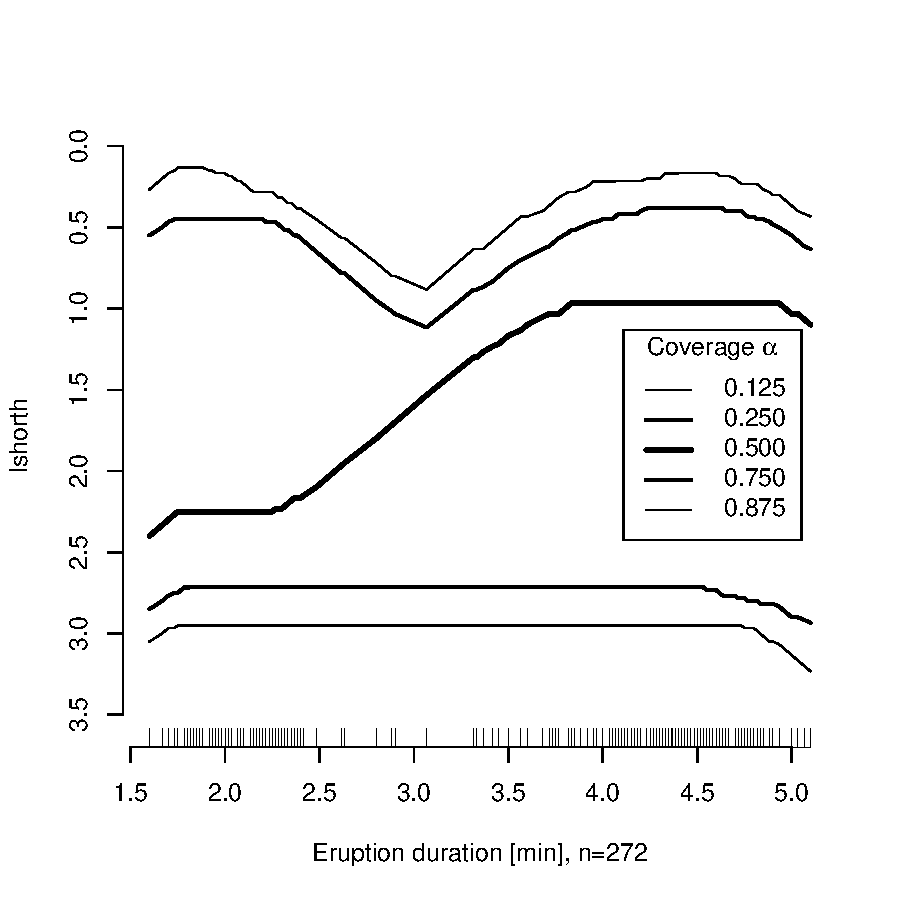
\includegraphics[width=0.45\linewidth]{TheShorthPlot-Faithful}
\caption{(left) Eruption durations of the Old Faithful geyser:  density estimation (R defaults)}\label{fig:faithfuldens}\caption{(right) Eruption durations of the Old Faithful geyser:  shorth plot}\label{fig:faithful}
\end{figure}

The contours of the shorth plot for high coverage levels $(\alpha > 50\%)$ just show the overall 
range of the data. The $50\%$ level indicates a pronounced skewness. The top levels 
($25\%, 12.5\%$) reveal 
that we have two modes, with a comparable coverage range. This is not obvious from 
the density plot, since the density plot mixes information about local heights attributable 
to modes with information about the mixture proportions.\gsnote{figure added to illustrate this} Density estimators with varying bandwidth or histograms with varying parameters could reveal these details (see figure \ref{fig:faithfuldensadj}). The multi scale property of the shorth plot allows to combine the aspects in one picture.
\begin{figure}[htb]
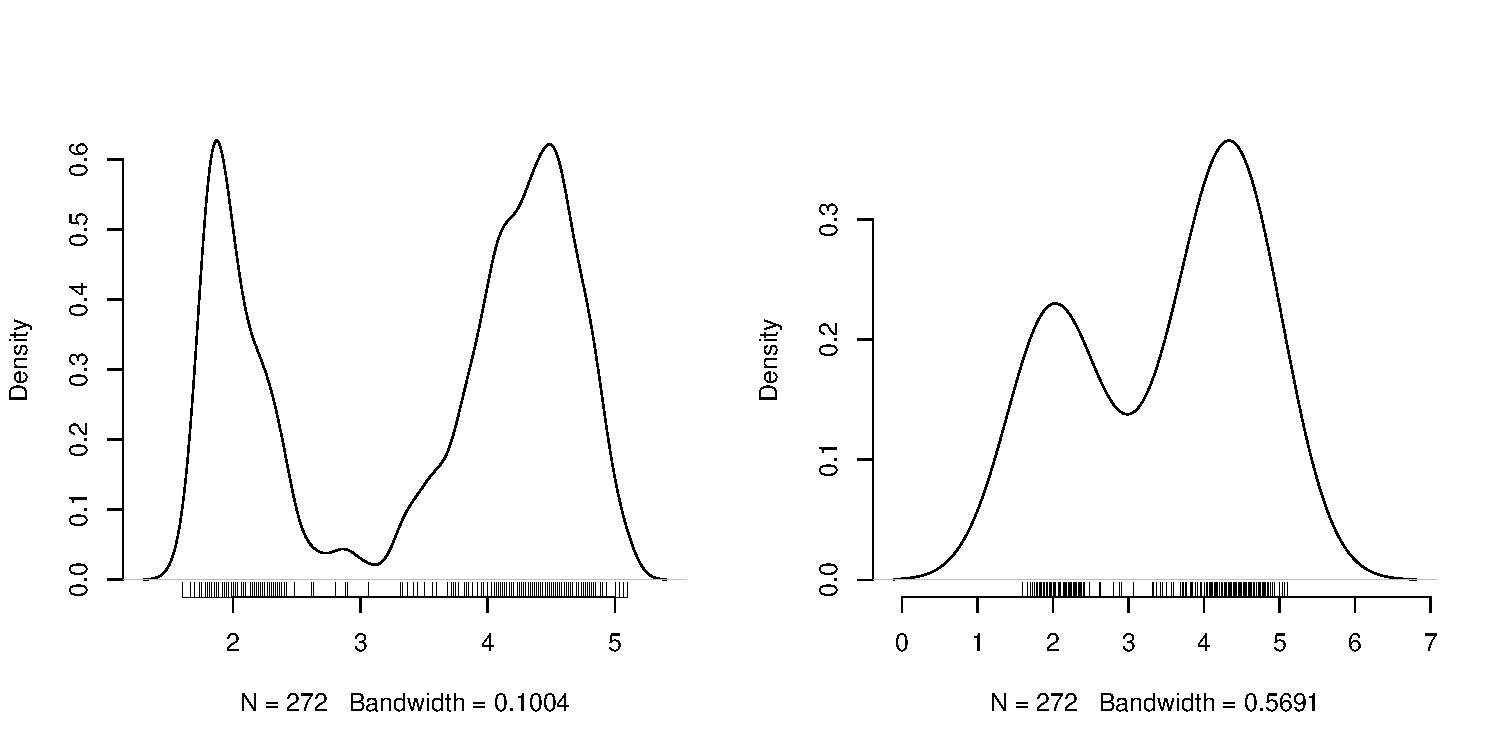
\includegraphics[width=0.95\linewidth]{TheShorthPlot-Faithfuldensadj}
\caption{Eruption durations of the Old Faithful geyser:  density estimation with varying bandwidth. The density plot mixes information about local heights attributable 
to modes with information about the mixture proportions. }\label{fig:faithfuldensadj}
\end{figure}

%
%\clearpage
%
\subsection{Melbourne Temperature Data}
%
R. Hyndman pointed out the bifurcation to bimodality in the Melbourne temperature data set \cite{Hyndman1996Estimating-and-}. We use an extended version of the data set\footnote{Melbourne temperature data 1955-2007, provided by the Bureau of Meteorology, Victorian Climate Services Centre, Melbourne.} and analyze the day by day difference in temperature   at 15h (the daily report reference time) conditioned on today's emperature and pressure at the reference time.  The shorth plot view is in figure \ref{fig:melbournet}. The full picture reveals a cusp-type bifurcation. Figure \ref{fig:melbourne} shows the shorth plot for the temperature difference at 15h (the daily report reference time) to next day's temperature, conditioned on today's temperature and pressure. It reveals the modality split as well as the skewness which is pressure dependent.
\begin{figure}[htb]
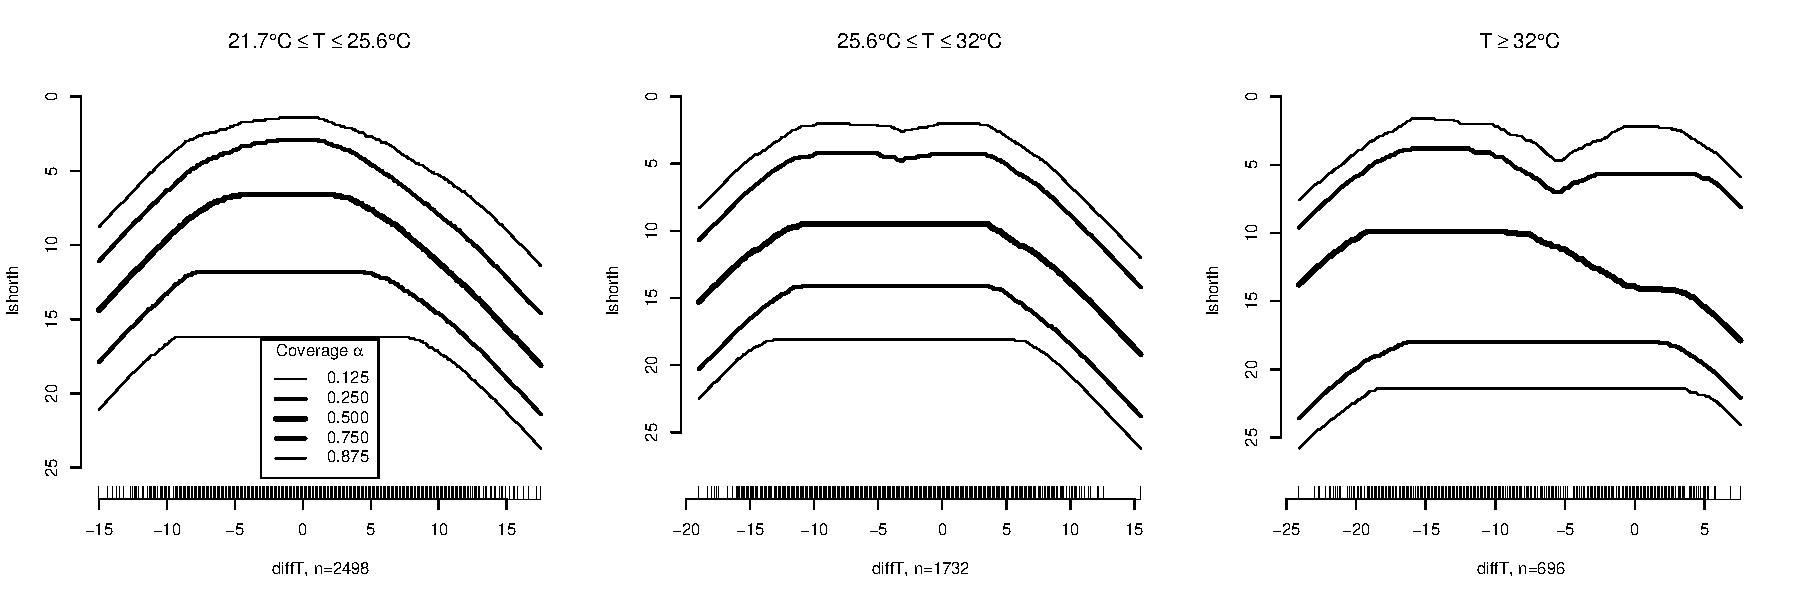
\includegraphics[width=\linewidth]{TheShorthPlot-MelbourneT}
%\caption{Eruption durations of the Old Faithful geyser: density estimation (R defaults)}\label{fig:faithfuldens}
%\end{figure}%
\caption{Shorth plot at coverage levels $\alpha =0.125,0.25,0.5,0.75,  0.875$ for Melbourne day by day temperature difference at 15:00h conditioned at today's temperature. 
A bifurcation to bimodality occurs at high temperatures.}\label{fig:melbournet}\end{figure}

%#	plotcond(tlim, plim=c(qpress[3],9999))
%#	plotcond(tlim, plim=c(qpress[2],qpress[3]))
\begin{figure}[htb]
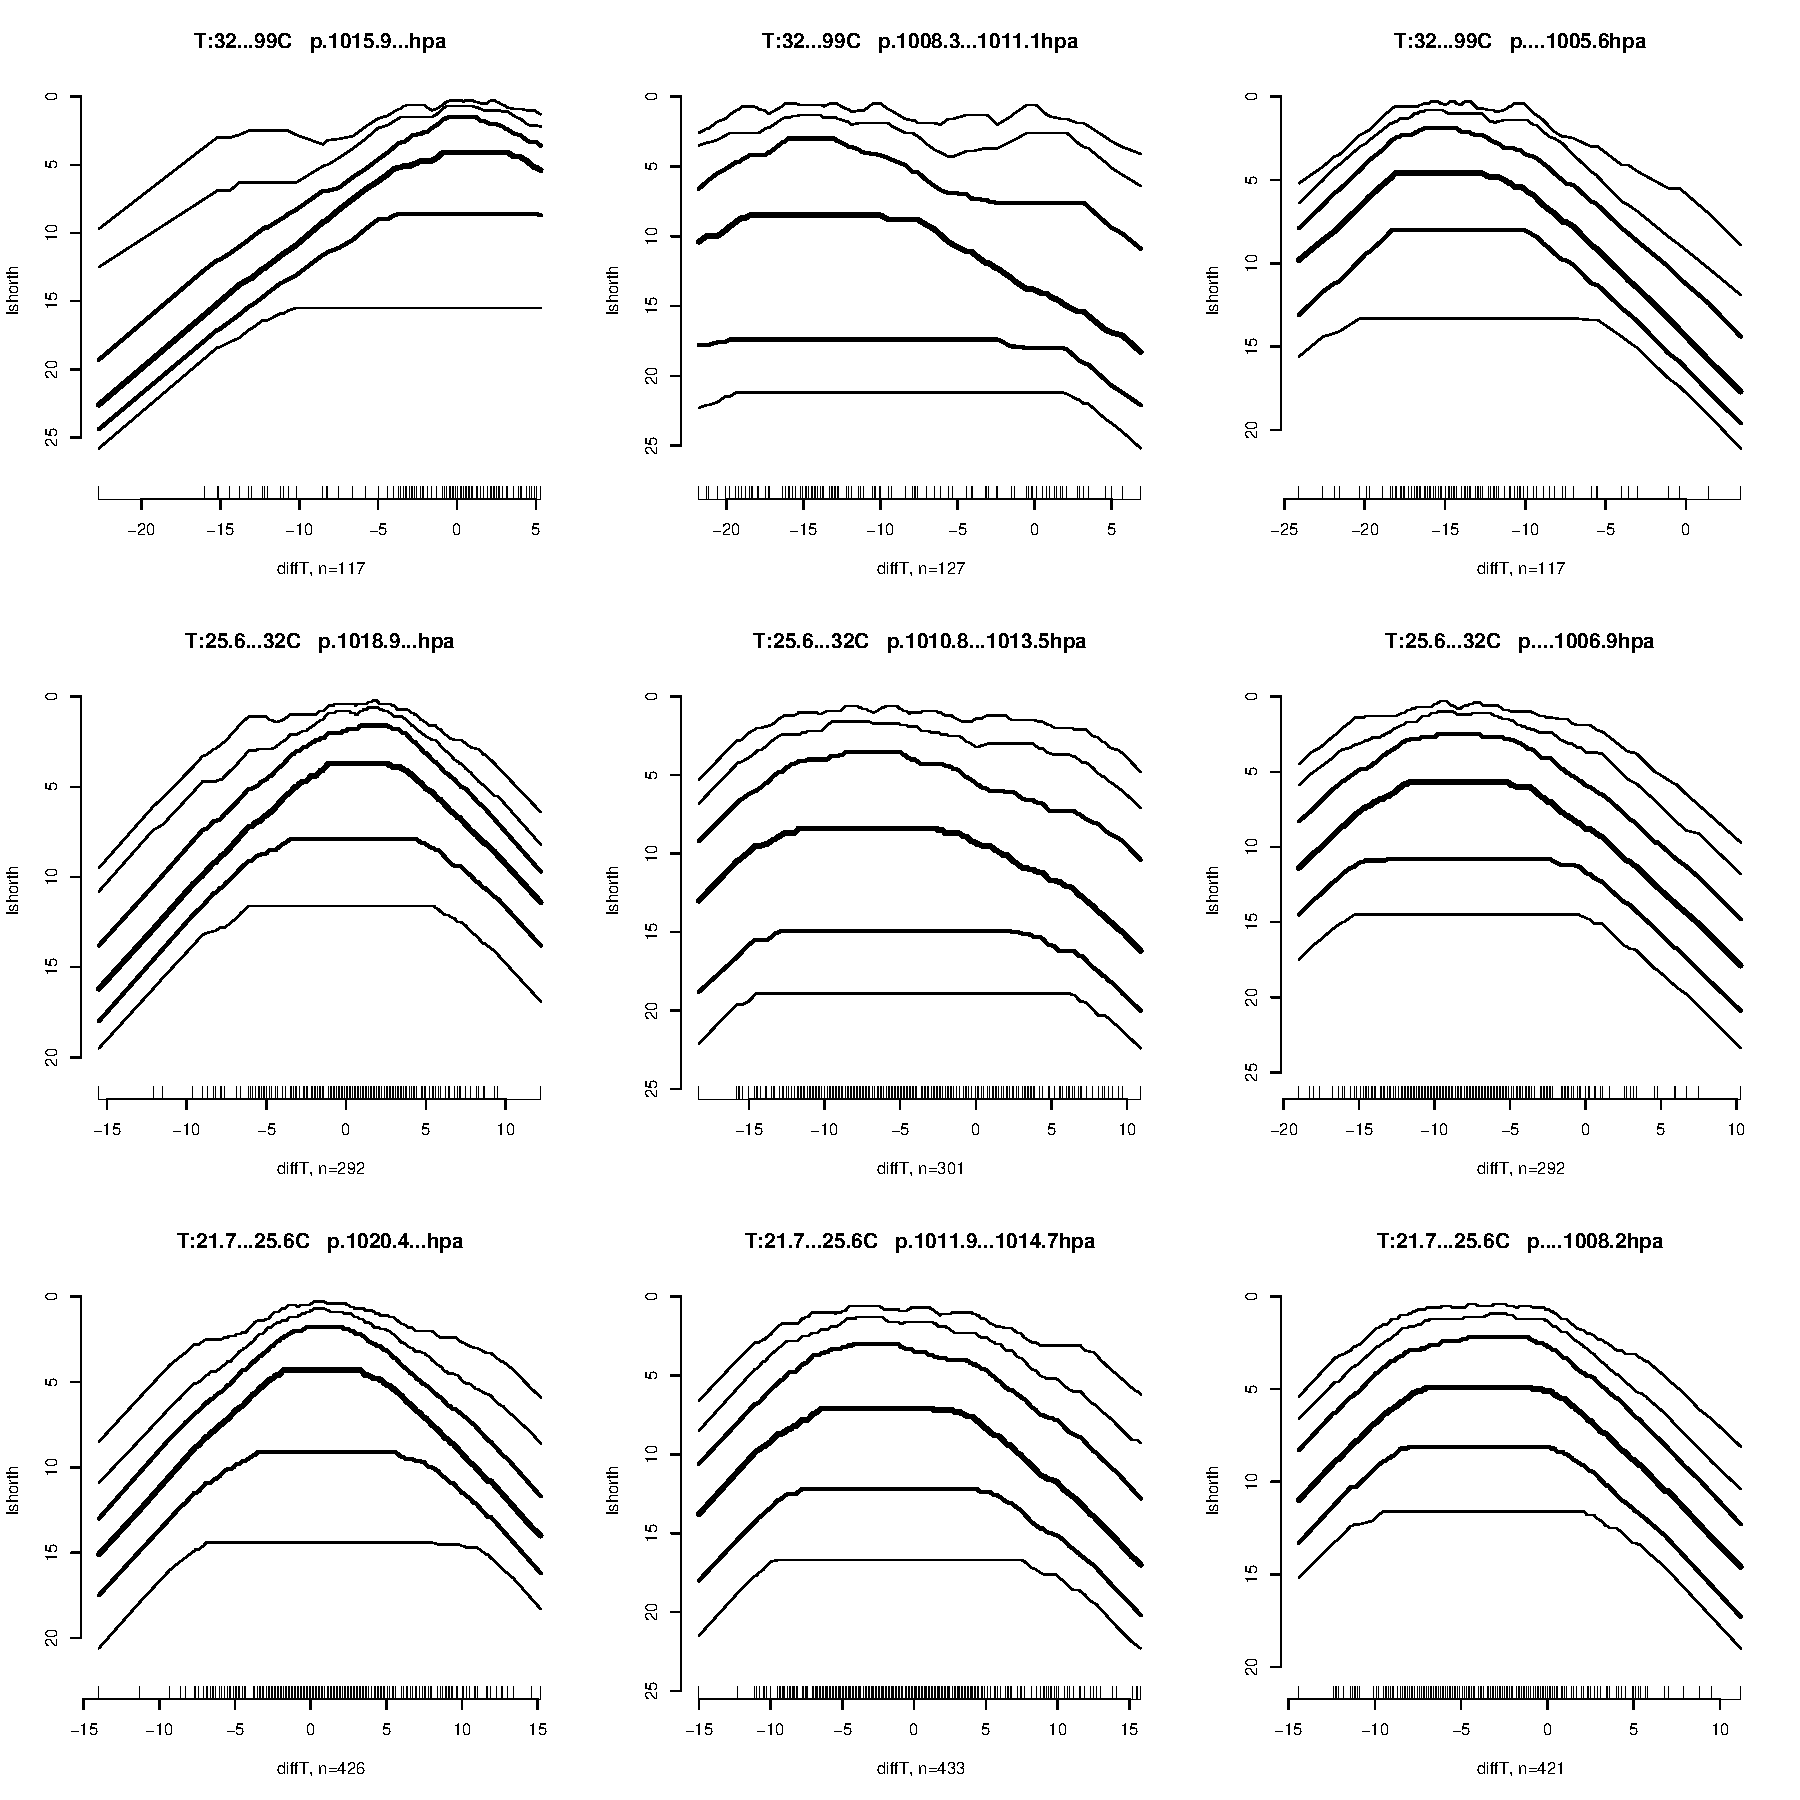
\includegraphics[width=\linewidth]{TheShorthPlot-Melbourne}
%\caption{Eruption durations of the Old Faithful geyser: density estimation (R defaults)}\label{fig:faithfuldens}
%\end{figure}%
\caption{Plot matrix of shorth plots for varying temperature ranges (vertical) and varying pressures (horizontal). Shorth plots at coverage levels $\alpha =0.125,0.25,0.5,0.75,  0.875$ for Melbourne day by day temperature difference at 15:00h,  conditioned at today's temperature and pressure. }\label{fig:melbourne}
\end{figure}


%
\subsection{Chondrite Data}
The  chondrite data set was used in to illustrate a strategy to hunt for modes in \cite{Good1980Density-estimat}. This data set is pressing the limits for the shorth plot since it has a very low sample size with presumably three modes  (see figure \ref{fig:chondrite}).

\begin{figure}[htb]
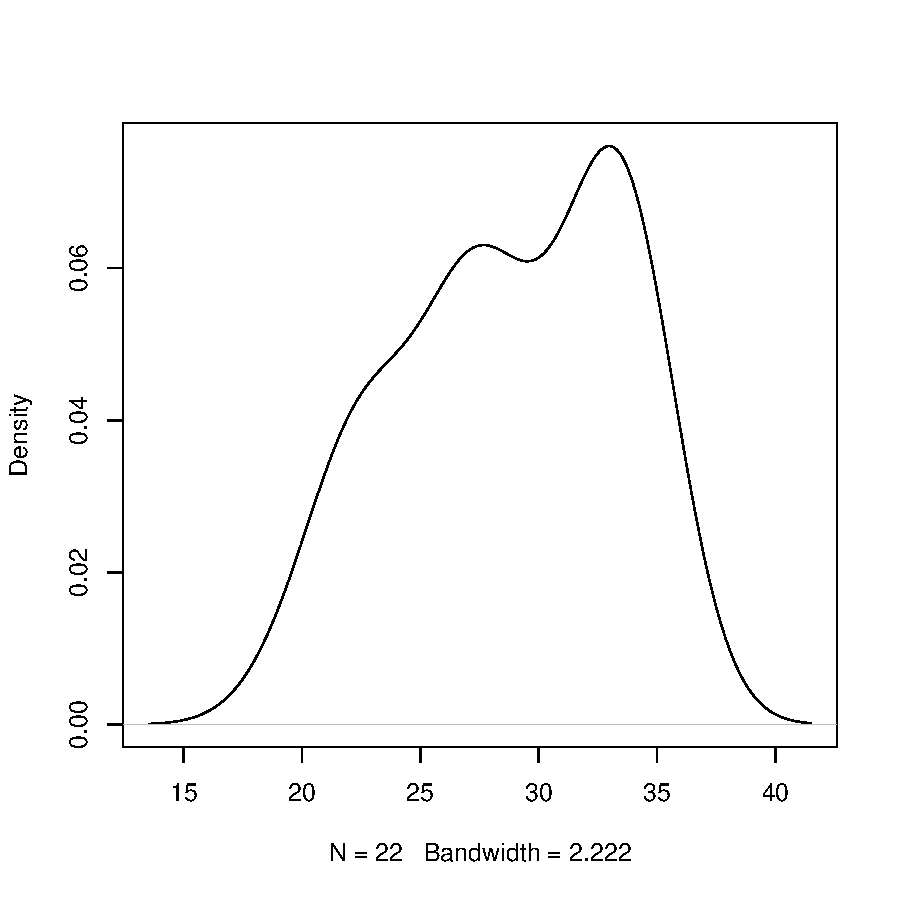
\includegraphics[width=0.45\linewidth]{TheShorthPlot-Chondritedens}
%\caption{Silicate in chondrite: density estimation}\label{fig:chondritedens}
%\end{figure}
%\begin{figure}[htb]
\hspace{\fill}
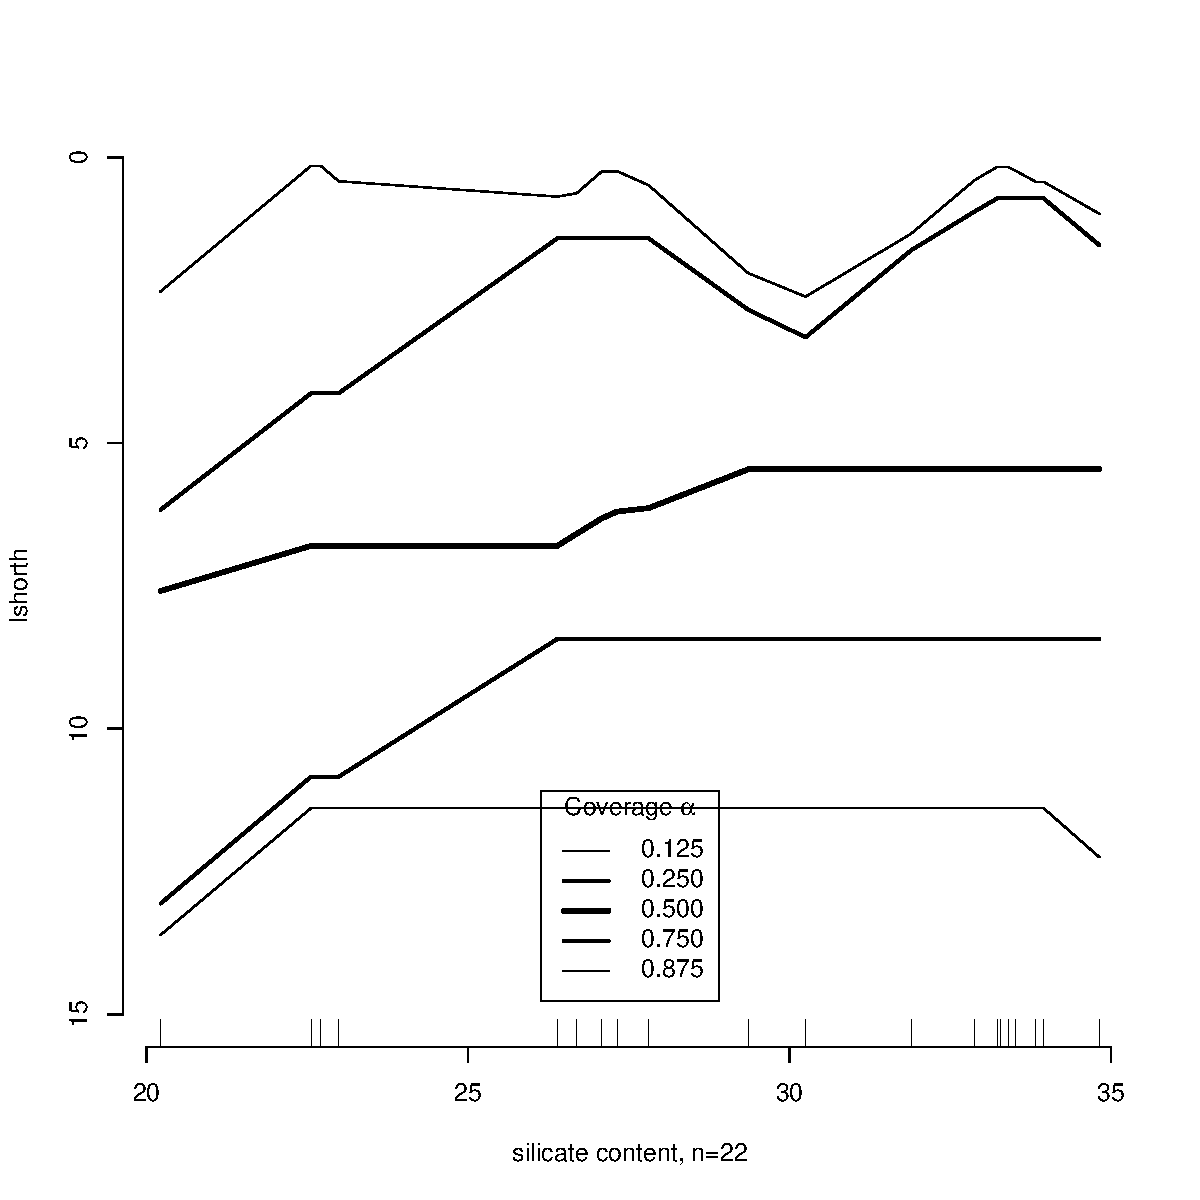
\includegraphics[width=0.45\linewidth]{TheShorthPlot-Chondrite}
\caption{(Left) Silicate in chondrite: density estimation}\label{fig:chondritedens}
\caption{(Right) Silicate in chondrite: shorth plot. Note: different scales are used.}\label{fig:chondrite}
\end{figure}
Using the methods of  \cite{Good1980Density-estimat} would allow to reveal a third mode, but it is subject to discussion whether this is over-using the data dependency. The shorth, as a general purpose method, gives figure \ref{fig:chondrite}. Of course it would be possible to isolate a third mode by 
including a smaller coverage level. 
%\begin{figure}[htb]
%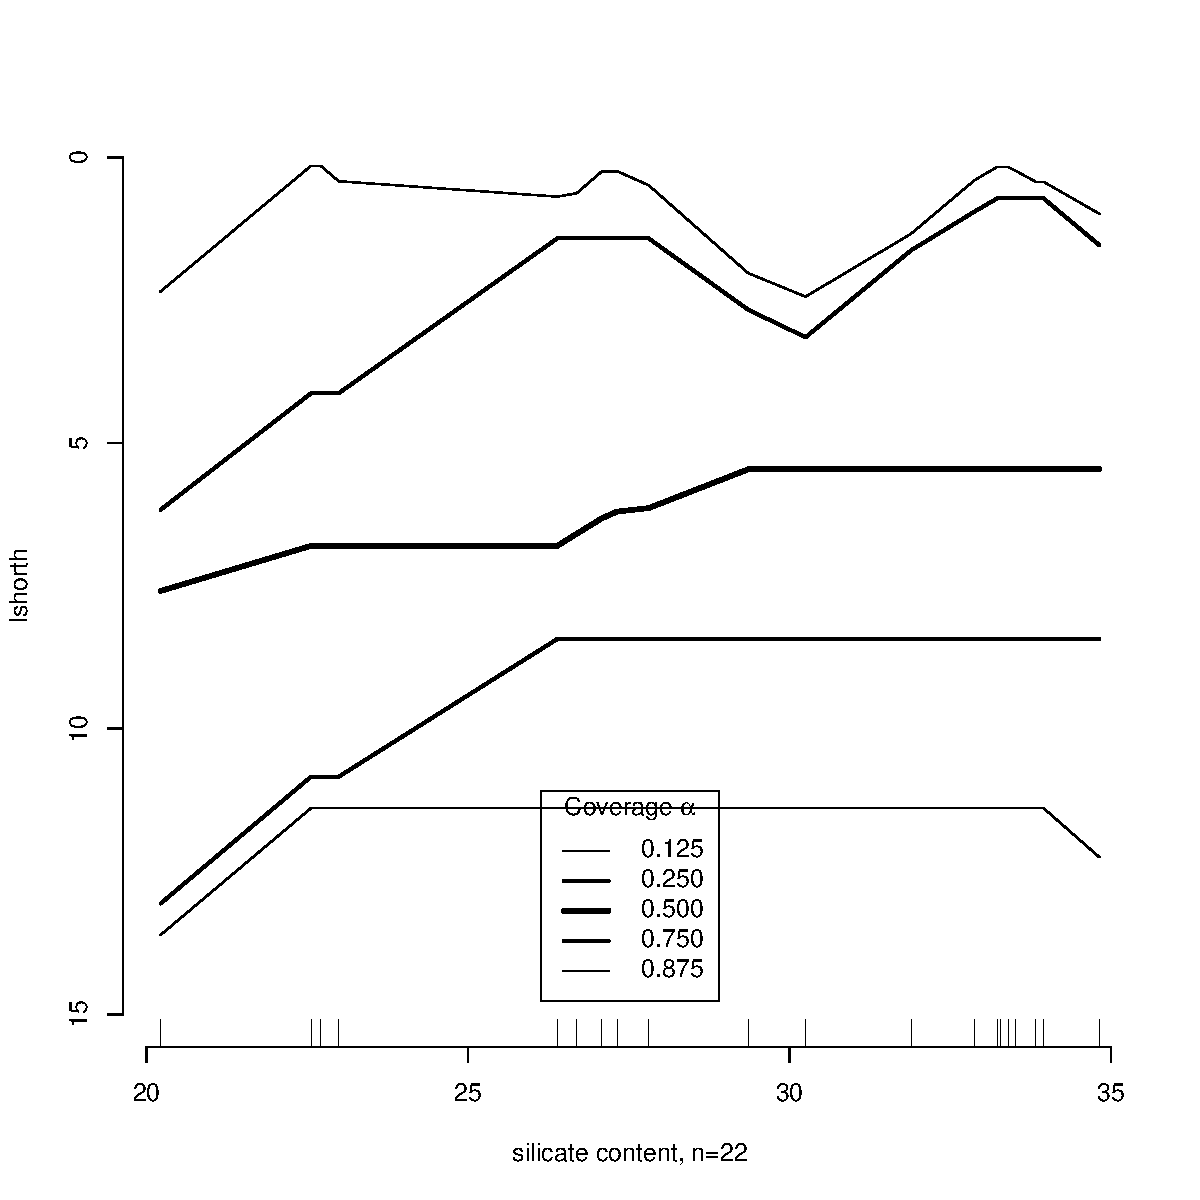
\includegraphics[width=0.5\linewidth]{TheShorthPlot-Chondrite}
%\caption{Silicate in chondrite: shorth plot}\label{fig:chondrite}
%\end{figure}

For comparison, we add the silhouette plot suggested in \cite{dwmgs91jasa} as figure \ref{fig:chondritesilh}. The silhouette plot, specialised at detecting modes, clearly outperforms the shorth plot for this extremely small data set. But although the short plot is  a general purpose plot,
 it hints at a third mode at all levels. If it goes to level $12.5\%$ it can trace the third mode, and clearly identifies it for lower coverage levels.%
\begin{figure}[htb]
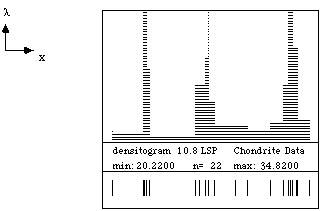
\includegraphics[width=0.5\linewidth]{../www/priv/graphics/excesschondrite1.jpg}

\caption{Silicate in chondrite: silhouette plot}\label{fig:chondritesilh}
\end{figure}
\clearpage
%
%
\subsection{Hartigan's Hat}
%
This example is a mixture in proportions $3:2:3$  of a uniform on $\left(0,\frac{1}{4}\right)$, on $\left(\frac{1}{4}, \frac{3}{4} \right)$, and on $\left(\frac{3}{4}, 1 \right)$ used in \cite{Hartigan1985The-dip-test-of} to illustrate the dip test of unimodality. See figure \ref{fig: hhat}. For a general analysis, it is a challenge because it combines bimodality with flat parts in the distribution, and a relatively low density in the ``dip''. Only $25\%$ of the distribution fall in the ``dip'', and thus it must be hidden in higher coverages for the shorth plot.

In this situation, kernel density estimation performs poorly, since it is heavily degraded by boundary effects which cannot cope with the flat parts of the distribution. The shorth plot hints at the flat parts on the outside, but has difficulties identifying the flat middle part.
%
\begin{figure}[htb]
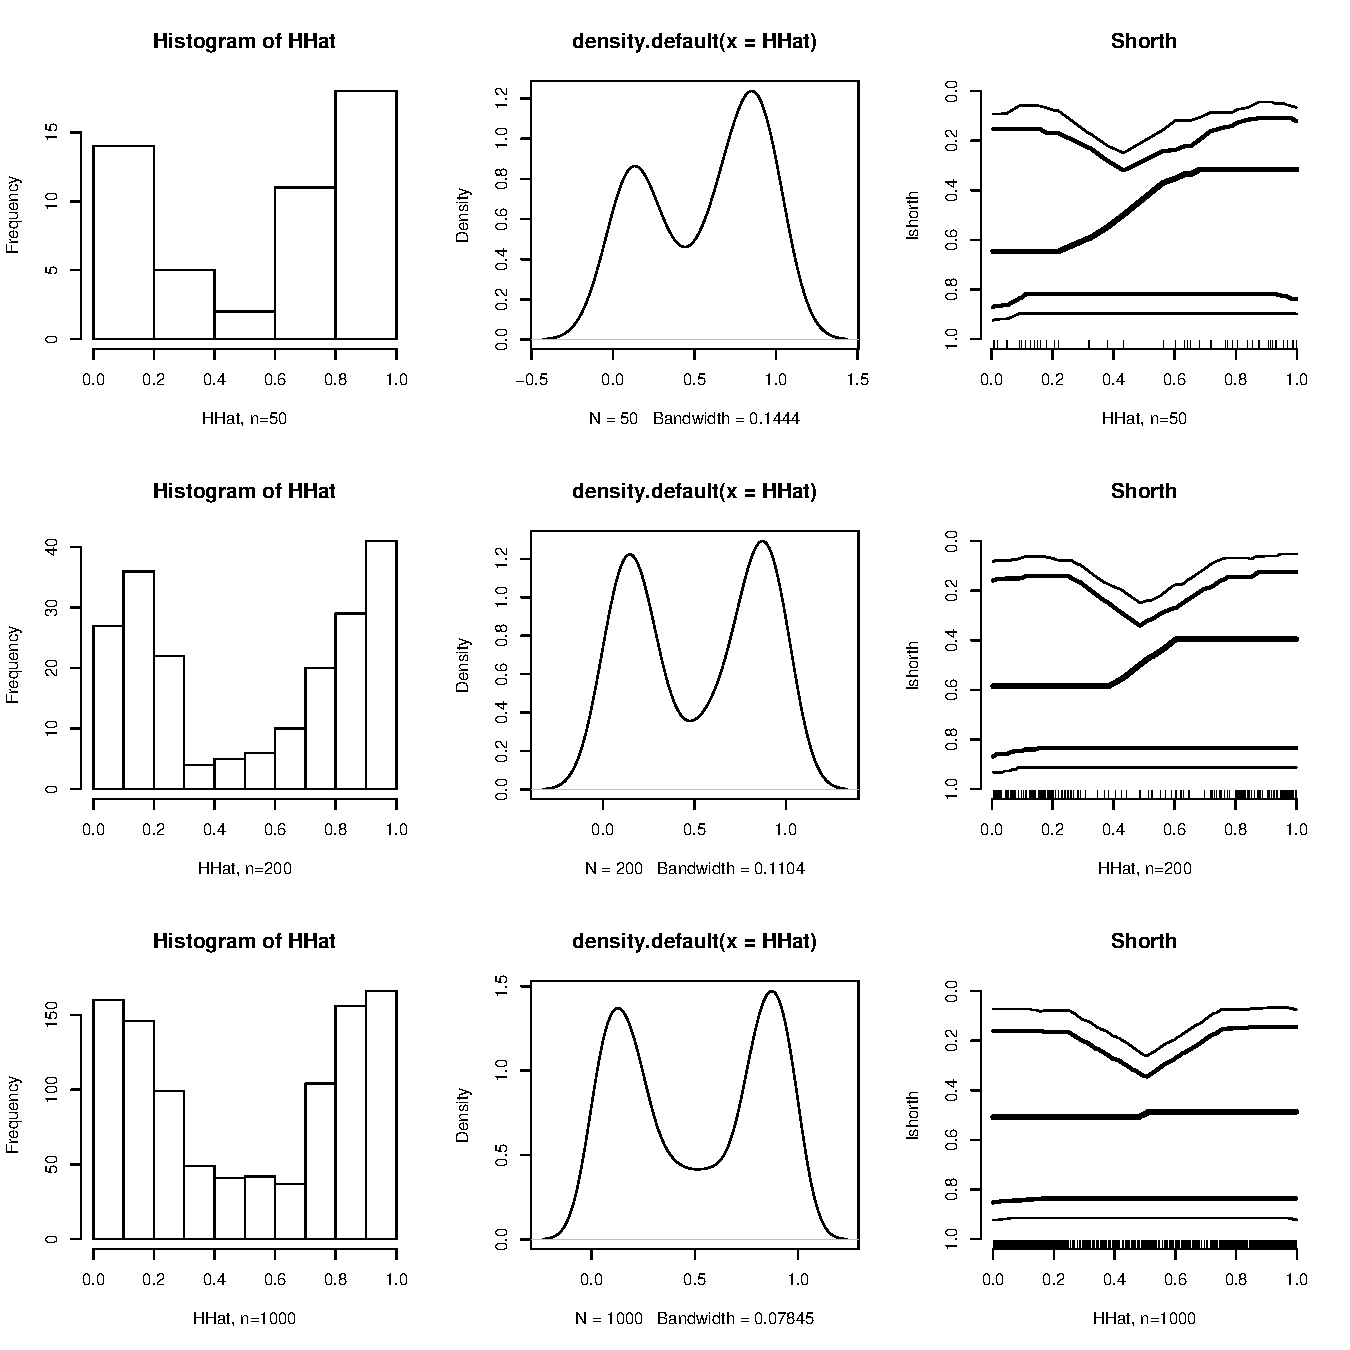
\includegraphics[width=0.9\linewidth]{TheShorthPlot-hhat}
\caption{Hartigan's Hat}\label{fig: hhat}
\end{figure}

%
\clearpage
%
\section{Extensions}
The shorth length is a well defined concept in one dimension. The generalisation to higher dimensions is the volume of a container covering a proportion of the data. In higher dimensions however there is no distinct class of containers to be considered. So additional choices have to be taken, such as using spheres or ellipsoids of minimal volume.

As with $QQ$-plots and $PP$-plots, the generalisation to the two sample case is immediate.

An open question is whether the shorth length approach can be carried over to a regression context.

\section{Related Approaches}
The shorth plot is related to kernel density estimation with variable bandwidth. It can be seen as a $k$-nearest neighbour approach. But in contrast to density estimation, it focusses on a concentration functional. Density is an infinitesimal concept. Mass concentration however is a local concept, but not an infinitesimal concept. As a consequence, density has no empirical counterpart, whereas mass concentration has. This makes the shorth length easier to handle for data analytical purposes.

\gsnote{added 20071028}
The shorth plot combines information on a series of coverage levels. For smoothed density estimators, it would be necessary to use a series of bandwiths. But even using  a series of bandwiths, the density estimators would not easily reveal the features which are apparent in the shorth plot.

The relation to mass concentration is shared with the silhouette and the excess density plot  (\cite{dwmgs91jasa}) or Hyndman's highest density regions (\cite{Hyndman1996Computing-and-G}). The view however is complementary. Silhouette and the excess density focus on concentration, but the shorth on local spread. Silhouette and the excess density  target at detecting modality and are model based for a global model (e.g., unimodal vs. bimodal). The shorth however has a local perspective, and is model independent.

P. A. and J. W. Tukey suggested a ``balloon plot'' in \cite{Tukey1981Data-Driven-Vie} (in \cite{Barnett1981Looking-at-mult}, reprinted in \cite{Tukey1988collected-V}). This is most closely related to the shorth plot. The main difference is that the balloons are centred at data points. The shorth plot does not use this centring, thus avoiding unnecessary random fluctuation.

The SIzer approach by Chaudhuri and Marron \cite{Chaudhuri1999SiZer-for-Explo} is related in spirit to the shorth plot. It tries to present a multiscale representation for smoothing while controlling the artifacts of smoothing by going to a probability scale. The shorth plot avoids the initial smoothing step and is strictly data based.



\section{Summary}
The shorth plot is a means to investigate mass concentration. 
It is easy to compute, avoids the bandwidth selection problems, and allows scanning for local as well
as for global features of the distribution. The good rate of convergence of the shorth estimator makes it useful already at moderate sample sizes.

%\section{}
%\subsection{}
%\backmatter
%\bibliographystyle{alpha}
\bibliographystyle{amsalpha}
%\bibliographystyle{alphadin}
%\bibliographystyle{agsm}
%\bibliographystyle{amsxport}
%\bibstyle{alpha}
%\pagenumbering[Bibliography]{bychapter}% no effect
\bibliography{/Users/gs/Documents/lectures/src/shared/bib/sda}

\ifx\private\undefined%
\else
\printindex
\fi

\ifx\private\undefined%
\else
\noindent
{\tiny%
\verb|$URL: svn+ssh://gsawitzki@svn.r-forge.r-project.org/svnroot/lshorth/Rnw/TheShorthPlot.Rnw.tex $|\\
\verb+$Revision: 44 $+\\
\verb+$Id: TheShorthPlot.Rnw.tex 44 2007-10-07 20:01:08Z gsawitzki $+
}
\fi

\end{document}
